\documentclass[10pt,tikz,border=1mm]{standalone} 
\usepackage{mathpazo}
\usepackage[T1]{fontenc}
\usetikzlibrary{positioning,calc,arrows.meta}
\begin{document}
	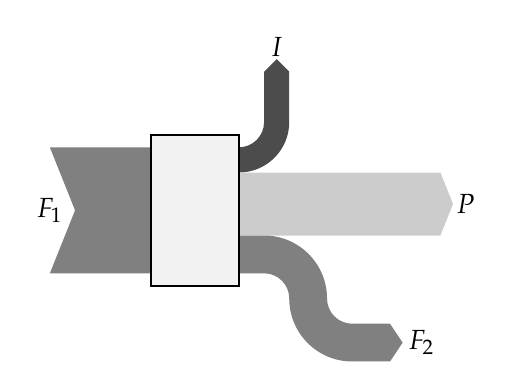
\begin{tikzpicture}[scale=0.16]
	%\draw[step=1cm,black!20,very thin] (0,-15) grid (35,15);
	\draw[fill=black!50,draw=none] (0,5)--(8,5)--(8,-5)--(0,-5)--(2,0)--cycle;	
	\draw[fill=black!70,draw=none] (15,5) arc(270:360:2cm) -- (17,11) -- (18,12) -- (19,11) -- (19,7) arc(0:-90:4cm)--cycle;
	\draw[fill=black!20,draw=none] (15,3) -- (31,3) --(32,0.5) -- (31,-2) -- (15,-2) -- cycle;
	\draw[fill=black!50,draw=none] (15,-2) -- (17,-2) arc(90:0:5cm) arc(180:270:2cm) -- (27,-9) -- (28,-10.5) -- (27,-12)--(24,-12) arc(270:180:5cm) arc (0:90:2cm) -- (15,-5) -- cycle;
	\draw[fill=black!5,thick] (8,-6) rectangle (15,6);
	\node at (0,0) {$F_1$};
	\node at (18,13) {$I$};
	\node at (33,0.5) {$P$};
	\node at (29.5,-10.5) {$F_2$};
	\end{tikzpicture}
\end{document}	

